\documentclass[authoryear, twocolumn]{elsarticle}
\usepackage{lmodern}
\usepackage{amssymb,amsmath}
\usepackage{ifxetex,ifluatex}
\usepackage{fixltx2e} % provides \textsubscript
\ifnum 0\ifxetex 1\fi\ifluatex 1\fi=0 % if pdftex
  \usepackage[T1]{fontenc}
  \usepackage[utf8]{inputenc}
  \usepackage{eurosym}
\else % if luatex or xelatex
  \ifxetex
    \usepackage{mathspec}
  \else
    \usepackage{fontspec}
  \fi
  \defaultfontfeatures{Ligatures=TeX,Scale=MatchLowercase}
  \newcommand{\euro}{€}
\fi
% use upquote if available, for straight quotes in verbatim environments
\IfFileExists{upquote.sty}{\usepackage{upquote}}{}
% use microtype if available
\IfFileExists{microtype.sty}{%
\usepackage{microtype}
\UseMicrotypeSet[protrusion]{basicmath} % disable protrusion for tt fonts
}{}
\usepackage[unicode=true]{hyperref}
\hypersetup{
            pdftitle={The link between tongue root advancement and the voicing effect: an ultrasound study of Italian and Polish},
            pdfauthor={Stefano Coretta},
            pdfborder={0 0 0},
            breaklinks=true}
\urlstyle{same}  % don't use monospace font for urls
\usepackage{natbib}
\bibliographystyle{plainnat}
\usepackage{graphicx,grffile}
\makeatletter
\def\maxwidth{\ifdim\Gin@nat@width>\linewidth\linewidth\else\Gin@nat@width\fi}
\def\maxheight{\ifdim\Gin@nat@height>\textheight\textheight\else\Gin@nat@height\fi}
\makeatother
% Scale images if necessary, so that they will not overflow the page
% margins by default, and it is still possible to overwrite the defaults
% using explicit options in \includegraphics[width, height, ...]{}
\setkeys{Gin}{width=\maxwidth,height=\maxheight,keepaspectratio}
\IfFileExists{parskip.sty}{%
\usepackage{parskip}
}{% else
\setlength{\parindent}{0pt}
\setlength{\parskip}{6pt plus 2pt minus 1pt}
}
\setlength{\emergencystretch}{3em}  % prevent overfull lines
\providecommand{\tightlist}{%
  \setlength{\itemsep}{0pt}\setlength{\parskip}{0pt}}
\setcounter{secnumdepth}{5}
% Redefines (sub)paragraphs to behave more like sections
\ifx\paragraph\undefined\else
\let\oldparagraph\paragraph
\renewcommand{\paragraph}[1]{\oldparagraph{#1}\mbox{}}
\fi
\ifx\subparagraph\undefined\else
\let\oldsubparagraph\subparagraph
\renewcommand{\subparagraph}[1]{\oldsubparagraph{#1}\mbox{}}
\fi

% set default figure placement to htbp
%\makeatletter
%\def\fps@figure{htbp}
%\makeatother

\frenchspacing
\usepackage{cleveref}
\setcitestyle{aysep={},notesep={:},citesep={,}}
\usepackage{ctable}

\title{The link between tongue root advancement and the voicing effect: an
ultrasound study of Italian and Polish}
\author{Stefano Coretta}
\date{08/09/2017}

\begin{document}
\maketitle

\section{Introduction}\label{introduction}

It is known that the root of the tongue can play a role in maintaining
voicing during the closure of voiced obstruents. The production of vocal
fold vibration requires a pressure differential between the sub-glottal
and the supra-glottal cavities (with lower pressure in the supra-glottal
cavity). During the production of voiced obstruents, the pressure in the
supra-glottal cavity quickly increases, due to the additional air
injected from the lungs in the supra-glottal cavity, which is completely
sealed in obstruent consonants. Such pressure increase can hinder the
ability to maintain voicing during closure, at the point that voicing
can stop if the lowest threshold of pressure differential is reached and
surpassed. \citet{westbury1983} argued that one way to counterbalance
the pressure increase in the supra-glottal cavity is to enlarge the
cavity through expansion of the pharyngeal walls. One way to achieve
this is to advance the root of the tongue. \citet{ahn2016} has recently
has demonstrated, drawing from ultrasound tongue imaging, that the root
of the tongue is advanced during the articulation of voiced consonants
in American English. She also showed that tongue root advancement is
present even when vocal fold vibration is not present during closure in
underlyingly voiced stops. An interesting question arising from the
connection between voicing and tongue root is weather the advancement of
the root is correlated with other phonetic characteristics, like the
duration of vowels preceding obstruents.

An extensive pool of studies showed that vowels tend to be longer when
followed by voiced obstruents and shorter when followed by voiceless
obstruents \citep{house1953, chen1970, klatt1973, lisker1973}. Most of
the literature on the topic suggests that different languages show
different magnitudes of such durational differential, and that in some
other languages the duration of vowels is not affected by the voicing of
the following
obstruent.\footnote{For a different opinion on the first matter, see @laeufer1992.}
Although several attempts have been put forward to explain the effect of
voicing on vowel durations, no consensus has been reached to date.
Nonetheless, a recurrent theme focusses on the differences that
characterise the gestural implementation of voiced and voiceless
stops.\footnote{However, see @javkin1976 and @kluender1988 for two perceptually inclined proposals.}
One of the earliest articulatory accounts of the voicing effect
attributed the difference in vowel duration to the divergent
configuration of the vocal folds in sonorant and obstruent voicing
\citetext{\citealp{halle1967}; \citealp[reiterated in][]{chomsky1968}}.
According to \citet{halle1967}, voicing in obstruents is produced with a
state of the glottis that is different from the configuration necessary
to produce vocal fold vibration in sonorants like vowels. On the
contrary, they claim that voiceless stops do not require any specific
glottal configuration and thus the voicing perpetuated during the vowel
can just naturally ceases at closure (or a few milliseconds thereof).
The authors thus hypothesise that, to allow the glottal state to change
from sonorant voicing to obstruent voicing, the vowel is lengthen so
that enough time is available for the change to happen. Although such
account seemed promising at the time it was proposed, later studies
failed to demonstrate that obstruent voicing is any different from
sonorant voicing.

Given the connection between voicing and tongue root advancement, it is
natural to ask whether tongue root advancement is also linked to vowel
duration. If this is indeed the case, then one would expect tongue root
advancement to play a role in language that have the voicing effect, but
not in languages that do not show it.

To test this hypothesis, I conducted an acoustic and articulatory study
that looked at vowel duration and tongue contours to assess the possible
link between consonantal and vocalic tongue gestures.

Tongue root advancement differences seems like a promising area of
enquiry since its link to voicing has been already confirmed. On the
same line of the laryngeal hypothesis, I put forward a similar account
in which it is tongue root advancement rather than fold configuration
that requires extra time during the vowel to be implemented. If tongue
root advancement plays a role in determining the duration of preceding
vowels through the extension mechanism described before, than one
expects languages with the voicing effect to show a systematic
advancement of the tongue root in voiced stops. On the contrary, tongue
root advancement in languages without the voicing effect should be
absent or less systematic.

Italian has been reported to have the voicing effect.
\citet{farnetani1986}, in a study assessing general properties on
segmental durations of spoken Italian, found for the pair of nonce words
/lata/ \textasciitilde{} /lada/ that the vowel /a/ was on average 35
msec longer when followed by the voiced stop /d/ (/lata/ 223 msec, sd =
18; /lada/ 258 msec, sd = 13, p.~26). \citet{esposito2002} extended the
research to all vowels and stops and found that vowels were longer when
followed by a voiced stop. Although the estimates from the statistical
models are not reported in the paper, judging from the figures in the
graphs, an average of 30-35 msec difference was found, which is similar
to what has been reported by \citet{farnetani1986}.

On the other hand, \citet{keating1984} reported that vowels in Polish
are not affected by the voicing of the following consonant. She tested
vowel duration in the word pair /rata/ \textasciitilde{} /rada/ and
found that there was a durational difference of 2 milliseconds. As for
the some of the Italian studies, statistical analysis was not performed,
although judging by the size of the difference, it can be assumed that
it is not significant.

\section{Methodology}\label{methodology}

\subsection{Participants}\label{participants}

Four native speakers for each of Italian and Polish have been recruited
on a volunteering basis in Manchester and in Italy. This research has
obtained ethic clearance by the University of Manchester (REF
2016-0099-76). The participants received a monetary compensation of
£10/10\euro{}.

\subsection{Equipment set-up}\label{equipment-set-up}

\begin{figure}
\centering
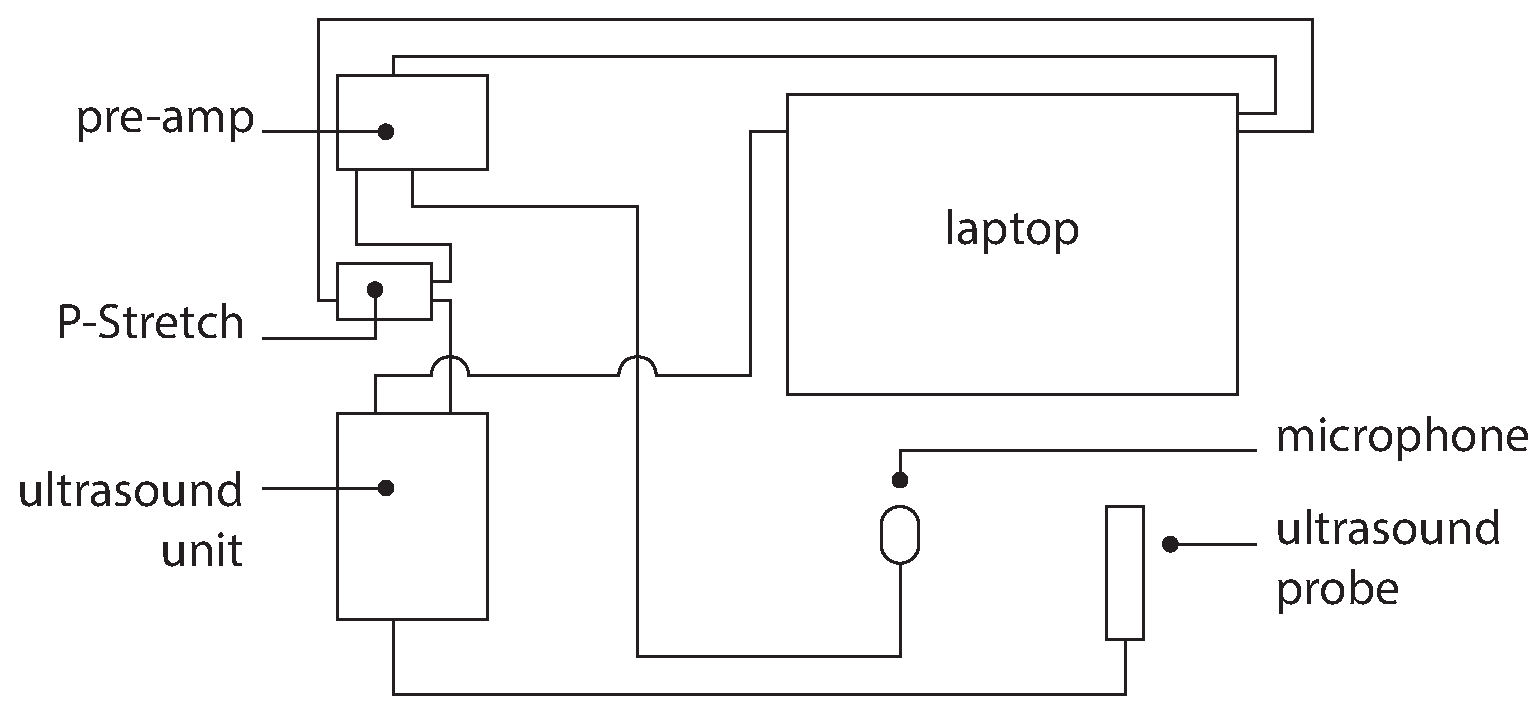
\includegraphics[width=1.00000\textwidth]{../../graphics/uti-setup.pdf}
\caption{Schematic representation of the equipment setup
(\citealt{articulate2011}, se text for details).\label{f:uti-setup}}
\end{figure}

An Articulate Instruments Inc. set-up was used for this study
(\Cref{f:uti-setup}). This is constituted by a TELEMED C3.5/20/128Z-3
(20mm radius, 2-4 MHz) ultrasonic transducer plugged into a TELEMED Echo
Blaster 128 unit. A synchronisation unit (P-Stretch) was plugged into
the Echo Blaster unit and used for automatic audio/ultrasound
synchronisation. A Movo LV4-O2 Lavalier microphone plugged into a
FocusRight pre-amplifier was used for audio recording. Articulate
Assistant Advanced (AAA) v2.17.2 running on a Hawlett-Packard ProBook
6750b laptop with Microsoft Windows 7 was used for the acquisition of
the audio and ultrasonic signals. Stabilisation of the ultrasound probe
was ensured by using the stabilisation headset produced by Articulate
Instruments Inc.

\subsection{Materials}\label{materials}

Disyllabic words of the form
C\textsubscript{1}V\textsubscript{1}C\textsubscript{2}V\textsubscript{2}
were used as targets, where C\textsubscript{1} = /p/, V\textsubscript{1}
= /a, o, u/, and C\textsubscript{2} = /t, d, k, g/ (e.g. /pata/, /pada/,
/poto/, etc.). A bilabial stop /p/ was chosen as the first consonant to
reduce influence on the following vowel (although cf.
\citet{vazquez-alvarez2007}). Only coronal and velar stops were used as
target consonants since labial consonants cannot be imaged with
ultrasonography. All possible combinations were employed, yielding to a
total of 12 target words. The words were embedded in medial position
within a frame sentence. Prosodically similar sentences were used to
ensure comparability between languages. The frame sentence was
\emph{Dico X lentamente} `I say X slowly' for Italian, and \emph{Mówię X
teraz} `I say X now' for Polish.

\subsection{Procedure}\label{procedure}

The stimuli were randomised for each participant, but the order was kept
the same within participant due to software constraints. Each
participant repeated the list of randomised stimuli six times. The
participants' occlusal plane was obtained using a bite plate, and the
hard palate was imaged by asking the participant to swallow water
\citep{scobbie2011}. The frame rate of the acquisition of the ultrasonic
data varied between 55 and 65 frames per second (one frame every 18-15
milliseconds). The audio signal was recorded at 22050 MHz, 16-bit.

\subsection{Data processing}\label{data-processing}

Synchronisation of the ultrasonic and audio signal was achieved in
post-processing, using the built-in procedure in AAA. The data were then
subjected to force alignment using the SPASS force aligner
\citep{bigi2015}. The outcome of the automatic annotation was then
manually corrected, according to the criteria in \Cref{t:dur-measures}.
The onset of the target consonant burst (C2 burst) was detected
automatically employing a Praat implementation of the algorithm
described in \citet{ananthapadmanabha2014}. The duration of the
following intervals was then extracted from the acoustic landmarks using
an automated procedure in Praat: vowel duration (V1 onset to V1 offset),
consonant duration (V2 offset to C2 offset), closure duration (V2 offset
to C2 burst).

\ctable[caption = List of measurements as extracted from acoustics.,
label = t:dur-measures,
width=\textwidth
]{ll>{\raggedright}p{5cm}}{}{
\FL
\textbf{measure}               &                  & \textbf{criteria}                                                                                    \ML
vowel onset           & V1 onset         & appearance of higher formants in the spectrogram following the burst of /p/ (C1)            \NN
vowel offset          & V1 offset        & disappearance of the higher formants in the spectrogram preceding the target consonant (C2) \NN
consonant onset       & C2 onset         & corresponds to V1 offset                                                                    \NN
closure onset         & C2 closure onset & corresponds to V1 offset                                                                    \NN
consonant offset      & C2 offset        & appearance of higher formants of the vowel following C2 (V2)                                \NN
consonant burst onset & C2 burst         & automatic detection \citep{ananthapadmanabha2014}                                           \LL
}

Tongue contours were extracted from the ultrasonic data using Articulate
Assistant Advanced \citep[AAA,][]{articulate2011}. Spline lines were
first fitted to the visible contours using the batch tracking function
natively included in AAA. Manual correction was applied in the cases
where the automatic tracking showed clear errors. Tongue displacement
along time was thus calculated in AAA using a custom module provided by
Dr.~Patrycja Strycharczuk \citep{Strycharczuk2015}. The displacement was
calculated based on the movement of the splines along a given fan line.
For each speaker, two relevant fan lines were chosen: one for the tongue
tip and one for the tongue dorsum. The selection of the fan lines was
based on the inspection of the standard deviation of the splines in the
relevant area of the tongue. The fan line that showed the highest
standard deviation was then chosen as the relevant fan line for the
calculation of displacement. Velocity and tangential velocity were also
calculated. The time of maximum displacement based on tangential
velocity was finally obtained using a modified version of a search
set-up provided by Dr.~Patrycja Strycharczuk.

\subsection{Analysis}\label{analysis}

The coordinates of the splines were exported at acoustic closure and at
maximum displacement. The contours were normalised by applying
offsetting and rotation relative to the participant's occlusal plane
\citep{scobbie2011}. Generalised additive mixed effects models
\citep{wood2006} were used for the statistical analysis of tongue
contour data in R \citep{r-core-team2017}. Duration measurements were
subject to linear mixed effects models using \texttt{lme4} in R
\citep{bates2015}.

\section{Results}\label{results}

\subsection{Vowel duration and
voicing}\label{vowel-duration-and-voicing}

A linear mixed effect regression model was fit on the Italian vowel
durations with duration as the outcome variable, vowel quality (/a, o,
u/), voicing and place of articulation of the following consonant,
sentence duration as fixed effects, random intercepts by speaker and
word, and random slopes for voicing by speaker. An interaction between
voicing and vowel quality was also included, which turned out to be
significant. P-values were obtained through likelihood ration tests
comparing a model including voicing with a null model without voicing.
According to the model, Italian vowels are 19.5 msec (±5.5) longer if
followed by a voiced stop (\(\chi^2\)(3) = 18.5, p = 0.000337).

For Polish, the same model structure was used, excluding the
voicing-vowel interaction (which was not significant). Surprisingly, the
model reported a partially significant 8 msec (±3) effect of consonantal
voicing on the preceding vowel (\(\chi^2\)(1) = 5.4, p = 0.02). The
exploration of the random slopes by speaker showed that one speaker
showed a particularly higher slope for voicing, meaning that the effect
of voicing was stronger in his data. This observation will come handy
while discussing about the results of the tongue contour data.

\subsection{Tongue contours}\label{tongue-contours}

The Italian tongue contour analysis showed that voiced stops are
produced with advancement of the root of the tongue. Generalised
additive mixed effect models were fitted for each speaker: the
y-coordinates of the contours were the outcome variable; the
x-coordinates the parametric term; a reference smooth term for X, with
difference smooths for X by voicing, vowel quality, and place of
articulation of following consonant; random smooths by word. A
first-order autoregressive model was included, given the high
auto-correlation residuals as obtained by visual inspection of the
residuals. For two participants out of four, the root was significantly
more front in voiced stops in both vocalic contexts (/a, o/). On the
other hand, one participant had significant tongue root advancement only
following /a/, while the fourth participant didn't show advancement at
all. For Polish, three out of four speakers did not have tongue root
advancement, while the fourth speaker showed significant advancement in
both vocalic contexts.

Further contour analysis was carried out at the point of acoustic
closure for Italian and for the Polish speaker showing advancement.
Surprisingly, the tongue root in the voiced condition was found to be
already in advanced position at closure. Both the Italian (4 speakers)
and the Polish data (1 speaker) show that the root of the tongue at the
time of consonantal closure is advanced in both languages. Models fitted
on the individual speakers comparing tongue contours at closure and at
maximum displacement further confirmed that root advancement was bigger
at maximum displacement for Italian, but not for Polish.

\section{Discussion}\label{discussion}

The presence of tongue root advancement in Italian but not in Polish
initially supports the idea that vowels are longer if followed by voiced
stops to allow time for the root to reach a position suitable for
consonantal voicing. The reported absence of the voicing effect in
Polish could then be ascribed to the absence of tongue root advancement
in the voiced consonants of Polish. However, such statement is
complicated by two facts that emerged from the data analysed in this
study. First, tongue root advancement was found in one of the Polish
speakers and it was absent from one of the Italian speakers. Second,
even though the effect was not as big as for Italian, the Polish
duration data nonetheless showed a difference of 8 msec. However, as
mentioned above, one Polish speaker had a particularly higher slope for
voicing, and incidentally this is also the same and only Polish speaker
who showed root advancement. Moreover, a difference of 8 milliseconds
could be considered to be quite small in any case, although
statistically
detectable.\footnote{A model fitted on the data excluding the outlier speaker leads in fact to a smaller estimate of about 6 msec.}

The data also showed raising of the tongue dorsum concomitant to the
advancement of the root. Although such gesture was not prospected on the
basis of the tested hypothesis, it makes sense from an anatomical stand
point. Given the anteriorisation of the tongue root, other things being
equal, it derives that the tongue mass gets compressed. Such compression
can be counterbalanced (entirely or partially) by allowing the dorsum of
the tongue to raise. It is not thus surprising to observe a raised
dorsum in voiced stops accompanying root advancement.

\bibliography{linguistics.bib}

\end{document}
